% ---------------------------------------------------------------------------
% Golden Hour -- Informe final (Fase 5)
%
% Compilar:  pdflatex informe.tex && pdflatex informe.tex
% (dos pasadas: la primera resuelve las referencias cruzadas)
%
% Requisitos: una distribución LaTeX estándar (TeX Live, MiKTeX u Overleaf).
% Si el sistema no tuviera el paquete de castellano de babel, comentar la
% línea de \usepackage[...]{babel}: el documento compila igual, solo pierde
% la partición de palabras en español.
%
% Las tablas de report/tables/informe_*.tex y las figuras de report/figures/
% NO se editan a mano: las regenera `python run_fase5.py` a partir de los CSV
% de data/outputs/. Si un número de este informe no cuadra con el panel, la
% causa es que falta correr esa fase, no una discrepancia de criterio.
% ---------------------------------------------------------------------------
\documentclass[11pt,a4paper]{article}

\usepackage[utf8]{inputenc}
\usepackage[T1]{fontenc}
\usepackage[spanish,es-tabla,es-nodecimaldot]{babel}
\usepackage[margin=2.4cm]{geometry}
\usepackage{amsmath}   % \text{} dentro de fórmulas
\usepackage{graphicx}
\usepackage{booktabs}
\usepackage{array}
\usepackage{float}
\usepackage{xcolor}
\usepackage[font=small,labelfont=bf]{caption}
\usepackage{enumitem}
\usepackage[hidelinks]{hyperref}

\graphicspath{{figures/}}
\setlength{\parskip}{0.35em}
\setlength{\parindent}{0pt}
\setlist{itemsep=0.15em, topsep=0.25em}

\title{\vspace{-1.2cm}\textbf{Golden Hour}\\[0.25em]
\large Acceso por carretera a establecimientos de salud con capacidad
resolutiva en Piura, Ayacucho y Loreto}

% TODO: reemplazar por los nombres completos de los tres integrantes.
\author{Equipo del trabajo integrador}
\date{Setiembre de 2026}

\begin{document}
\maketitle
\vspace{-0.6cm}

\begin{abstract}
\noindent
Se estima el tiempo de viaje en automóvil hasta el establecimiento de salud
con capacidad resolutiva (categoría II-1 o superior) más cercano en Piura,
Ayacucho y Loreto. Sobre una muestra estratificada de 5{,}002 de 19{,}460
centros poblados, enrutada con OSRM sobre OpenStreetMap y ponderada por el
Censo 2017, el 71.8\,\% de la población llega en menos de 30 minutos y
708{,}676 personas (18.0\,\%) están a más de una hora. El promedio esconde
tres realidades: el tiempo medio ponderado es de 20.6 minutos en Piura, 67.2
en Ayacucho y 703.1 en Loreto. El Gini del acceso es 0.919 y la brecha
rural/urbana, de 2.3 veces. Solo 23 de 237 distritos tienen establecimiento
resolutivo propio. Los quince distritos con peor acceso están todos en
Loreto, donde el transporte real es fluvial: el principal hallazgo es también
la principal limitación del modelo.
\end{abstract}

% ===========================================================================
\section{Introducción y planteamiento del problema}
% ===========================================================================

En emergencias obstétricas, traumatismos y cuadros quirúrgicos agudos, lo que
determina el desenlace no es la existencia de un establecimiento de salud
cercano, sino la existencia de uno capaz de \emph{resolver} el cuadro. Una
posta de categoría I-1 atendida por un técnico no reemplaza a un hospital con
sala de operaciones. La pregunta que guía este trabajo es, por lo tanto,
deliberadamente estrecha:

\begin{quote}
\textbf{¿Cuánto tiempo le toma a la población de Piura, Ayacucho y Loreto
llegar por carretera al establecimiento de salud con capacidad resolutiva más
cercano, y qué tan desigualmente está repartido ese tiempo?}
\end{quote}

Los tres departamentos cubren las tres macrorregiones del país y permiten
contrastar una costa con red vial densa, una sierra de relieve accidentado y
una amazonía donde la red vial es marginal. La hipótesis de trabajo es que
cualquier promedio agregado oculta realidades incomparables entre sí, y que
una política formulada sobre ese promedio fallará justamente donde más falta
hace.

\textbf{Definición operativa de ``resolutivo''.} Se considera resolutivo todo
establecimiento de categoría II-1, II-2, II-E, III-1, III-2 o III-E del
Registro Nacional de IPRESS (RENIPRESS). Las categorías I-1 a I-4 (puestos y
centros del primer nivel) quedan fuera como destino: resuelven atención
primaria, no emergencias. La lista completa vive en \texttt{config.md} y se
puede cambiar sin tocar una línea de código.

\textbf{Umbrales.} Los cortes de 30, 60 y 120 minutos también salen de
\texttt{config.md}. Los 30 minutos corresponden a la noción clínica
convencional de que el tiempo prehospitalario debe mantenerse dentro de la
primera hora desde el evento --- la ``hora dorada'' ---, descontando el tiempo
de respuesta y de estabilización; los 120 minutos marcan el umbral a partir
del cual el traslado terrestre deja de ser una opción realista para una
emergencia.

% ===========================================================================
\section{Datos y fuentes}
% ===========================================================================

\begin{table}[H]
\centering
\caption{Fuentes, fecha de acceso y licencia. Las fechas de las descargas
automáticas las estampa el pipeline en \texttt{logs/download\_dates.json}.}
\label{tab:fuentes}
\footnotesize
\begin{tabular}{p{2.9cm}p{3.5cm}p{4.6cm}p{3.5cm}}
\toprule
Fuente & Contenido & Acceso & Licencia \\
\midrule
RENIPRESS (SUSALUD), Portal Nacional de Datos Abiertos
& Oferta: 3{,}718 establecimientos de los tres departamentos, con categoría,
condición y coordenadas
& \textbf{API automática fallida} (HTTP 418 a clientes no navegador);
descarga manual el 08/09/2026. Recurso actualizado por la fuente el
31/08/2026.
& Open Data Commons Attribution (ODC-By), declarada en el portal \\
\addlinespace
SIGMED (MINEDU), capa de centros poblados
& Demanda: 19{,}460 centros poblados con coordenada, altitud y nivel de
capitalidad
& \textbf{Sin API}: el portal exige aceptar condiciones y navegar un
formulario. Descarga manual el 08/09/2026.
& No declara licencia; solo condiciones de uso del aplicativo \\
\addlinespace
INEI, Directorio Nacional de Centros Poblados, Censos 2017 (Lib1541)
& Población censada por centro poblado, con código CCPP de 10 dígitos
& Automática, un \texttt{.xlsx} por departamento, 08/09/2026
& No declara licencia \\
\addlinespace
OpenStreetMap vía Geofabrik
& Red vial del Perú (\texttt{peru-latest.osm.pbf}, 244 MB)
& Automática, 08/09/2026
& ODbL 1.0 \\
\addlinespace
\texttt{juaneladio/\allowbreak peru-geojson}
& Límites distritales (cartografía censal INEI 2007)
& Automática, 08/09/2026
& MPL-2.0 \\
\bottomrule
\end{tabular}
\end{table}

Que dos de las cinco fuentes \emph{oficiales} no admitan descarga
programática es, en sí mismo, un resultado y no un contratiempo de plomería.
El módulo de adquisición no aborta cuando una fuente cae: registra el fallo
con su fecha en \texttt{logs/acquisition\_summary.json}, usa la copia local si
existe y continúa.

\textbf{Limitaciones conocidas de cada fuente.}
\begin{itemize}[leftmargin=1.3em]
\item \emph{RENIPRESS}: registro administrativo autodeclarado. El 23.45\,\% de
  los establecimientos no trae coordenadas y 390 no traen una categoría
  legible. Estar inscrito y ``en funcionamiento'' no garantiza dotación de
  personal ni de insumos.
\item \emph{SIGMED}: la propia página advierte que ``las coordenadas de
  centros poblados con servicio educativo han sido recopiladas de diversas
  fuentes con diferente nivel de precisión''. Además, el universo son centros
  poblados \emph{con servicio educativo}, lo que puede omitir asentamientos
  muy pequeños.
\item \emph{INEI 2017}: solo cubre centros poblados con código censal; el
  35.6\,\% de la demanda no lo tiene y queda sin población conocida. La suma
  del directorio para los tres departamentos, 3{,}356{,}495 habitantes,
  coincide con los totales departamentales publicados, lo que valida el cruce
  para la parte que sí empata.
\item \emph{OpenStreetMap}: cobertura desigual, mejor en zonas urbanas y peor
  en zonas rurales y amazónicas, donde además faltan las vías fluviales.
\item \emph{Límites distritales}: geometría censal de 2007, anterior a las
  creaciones distritales posteriores; un distrito de Piura llega con la
  geometría vacía.
\end{itemize}

% ===========================================================================
\section{Metodología}
% ===========================================================================

\subsection{Validación y limpieza}

Sobre la oferta se aplicaron seis reglas de calidad. Ninguna descarta
registros en silencio: cada fila marcada conserva su columna \texttt{flag\_*}
en \texttt{data/processed/}, y el reporte documenta cuántos registros se
marcaron, qué se hizo y por qué (tabla~\ref{tab:calidad-oferta}). Las mismas
seis reglas se aplicaron a la demanda, que llega mucho más limpia: 370 puntos
(1.9\,\%) caen fuera del polígono de su distrito declarado y se mantienen con
advertencia, porque sin verificación de campo no se puede saber si el error
está en la coordenada o en el ubigeo.

\begin{table}[H]
\centering
\caption{Reglas de calidad aplicadas a la oferta (RENIPRESS).}
\label{tab:calidad-oferta}
\footnotesize
\begin{tabular}{lrrp{5.4cm}}
\toprule
Regla & Marcados & \% del total & Acción \\
\midrule
coords\_faltantes & 872 & 23.45 & eliminado \\
fuera\_de\_bbox\_peru & 3 & 0.08 & mantenido con advertencia si es corregible por swap \\
lat\_lon\_intercambiados & 0 & 0.00 & corregido \\
fuera\_de\_su\_propio\_distrito & 355 & 9.55 & mantenido con advertencia \\
codigos\_duplicados & 0 & 0.00 & eliminado \\
encoding\_utf8\_vs\_latin1 & 1 & 0.03 & corregido in place en columnas de texto \\
\bottomrule
\end{tabular}

\end{table}

La población se empató por el código CCPP de 10 dígitos del Censo 2017. El
cruce cubre 12{,}509 de los 19{,}460 centros poblados (64.3\,\%); el resto
conserva \texttt{poblacion\_censada} nula y pesa cero en todo agregado
ponderado, en vez de recibir una población imputada.

\subsection{Enrutamiento}

Los tiempos se calculan con OSRM \cite{osrm} compilado sobre el extracto
peruano de OpenStreetMap, en tres perfiles (automóvil, bicicleta y a pie)
servidos por Docker. Para cada centro poblado de la muestra se calcula la
matriz \emph{completa} origen--destino contra todas las instalaciones
resolutivas --- no solo contra la más cercana en línea recta ---, porque la
más cercana en distancia euclidiana no es necesariamente la más cercana en
tiempo cuando hay un río o una cordillera de por medio. Esa matriz completa es
también lo que hace posible el simulador de escenarios de la sección
\ref{sec:simulador}.

\textbf{Muestreo.} Calcular la matriz para los 19{,}460 centros poblados es
innecesariamente caro, de modo que se tomó una muestra estratificada por
distrito de 5{,}002 puntos (25.7\,\% del universo, semilla fija 42). Todos los
agregados aplican el peso de diseño del muestreo además de la población
censada; sin ese peso, los distritos con muchos centros poblados pequeños
quedarían sistemáticamente subrepresentados.

\textbf{Enganche a la red vial.} Cada punto se proyecta al eje vial más
cercano dentro de un radio de 1{,}000 metros (tabla~\ref{tab:snapping}). El
38.3\,\% de los centros poblados muestreados no tiene ninguna vía transitable
en automóvil a esa distancia, mientras que el 100\,\% de los establecimientos
de salud sí la tiene: los establecimientos están donde están las carreteras;
buena parte de la población, no.

\begin{table}[H]
\centering
\caption{Enganche de los puntos a la red vial, por perfil.}
\label{tab:snapping}
\footnotesize
\begin{tabular}{llrrrr}
\toprule
Conjunto & Perfil & Puntos & Sin red vial & \% sin red vial & Distancia media (m) \\
\midrule
demanda\_muestreada & car & 5,002 & 1,914 & 38.3 & 199.7 \\
demanda\_muestreada & bike & 5,002 & 1,552 & 31.0 & 188.6 \\
demanda\_muestreada & foot & 5,002 & 1,551 & 31.0 & 188.6 \\
instalaciones\_resolutivas & car & 58 & 0 & 0.0 & 15.0 \\
\bottomrule
\end{tabular}

\end{table}

Para los 98 puntos (2.0\,\% de la muestra) sin ninguna ruta a un
establecimiento resolutivo existe un respaldo por distancia en línea recta
corregida por el factor de desvío empírico de la sección~\ref{sec:recta}. Las
filas así estimadas quedan marcadas y \textbf{no} entran en las métricas de
este informe, que las reporta aparte como ``sin acceso enrutable''.

\subsection{Métricas}

Para cada punto de demanda $i$ se define $t_i$ como el mínimo tiempo de viaje
hacia cualquier instalación resolutiva, y su peso efectivo como
$w_i = p_i \cdot d_i$, con $p_i$ la población censada 2017 y $d_i$ el peso de
diseño del muestreo. Sobre esa base se calculan: la distribución de población
por banda de tiempo; la media ponderada $\bar{t} = \sum w_i t_i / \sum w_i$
por distrito, provincia y departamento; la mediana ponderada; el ranking de
brechas críticas; el índice de Gini ponderado con su curva de Lorenz
\cite{lorenz,gini}; el contraste urbano/rural; y la correlación de Spearman
entre altitud y tiempo.

Un punto sin población conocida pesa cero y no entra al numerador ni al
denominador. Un punto sin ruta tampoco entra a la media, pero se reporta en
una categoría propia, para que un distrito con tiempo medio bajo y 30\,\% de
cobertura no se lea como bien servido.

\textbf{Clasificación urbano/rural.} El extracto de SIGMED no trae la variable
oficial de área urbana del INEI, definida por densidad de manzanas censales
contiguas. Se usó como aproximación la capitalidad político-administrativa: es
urbano el centro poblado que es capital de distrito, provincia o departamento.

\subsection{Panel interactivo y simulador de escenarios}
\label{sec:simulador}

El panel de Streamlit (\texttt{app.py}) presenta las mismas cifras en diez
pestañas y filtra por departamento, provincia, zona, categoría, institución y
umbral de tiempo. El panel \textbf{no reimplementa ninguna métrica}: al mover
un filtro vuelve a llamar a las funciones de \texttt{src/metrics.py} sobre el
subconjunto filtrado, de modo que panel e informe no pueden divergir. Un test
automatizado lo verifica comparando la tabla que recalcula el panel sin
filtros contra el CSV que cita este documento. El panel no llama a ningún
motor de enrutamiento: consume los parquet precalculados y abre en segundos.

El simulador permite ascender uno o más establecimientos I-3/I-4 existentes a
capacidad resolutiva y recalcula la cobertura como
$t^{\text{nuevo}}_i = \min(t_i,\ \min_{j \in A} t_{ij})$, donde $A$ es el
conjunto ascendido. Esta operación solo es posible porque Fase 2 guardó la
matriz completa y no únicamente la instalación más cercana.

% ===========================================================================
\section{Resultados}
% ===========================================================================

\subsection{Cobertura: el promedio esconde tres países}

\begin{table}[H]
\centering
\caption{Población estimada por banda de tiempo de acceso, en automóvil.}
\label{tab:cobertura}
\footnotesize
\begin{tabular}{lrr}
\toprule
Banda de acceso & Población estimada & \% de la población \\
\midrule
0-30 min & 2,828,176 & 71.78 \\
30-60 min & 353,536 & 8.97 \\
60-120 min & 291,933 & 7.41 \\
\textgreater{}120 min & 416,744 & 10.58 \\
sin ruta en la red vial & 49,811 & 1.26 \\
\bottomrule
\end{tabular}

\end{table}

El 71.8\,\% de la población representada llega en menos de media hora; leído
solo, ese número sugiere un sistema razonablemente accesible. La
figura~\ref{fig:cobertura} muestra por qué esa lectura es equivocada: al
desagregar, el mismo indicador va de 81\,\% en Piura a 35\,\% en Ayacucho, y
en Loreto el 32\,\% de la población necesita más de dos horas y un 8\,\%
adicional no tiene ninguna ruta.

\begin{figure}[H]
\centering
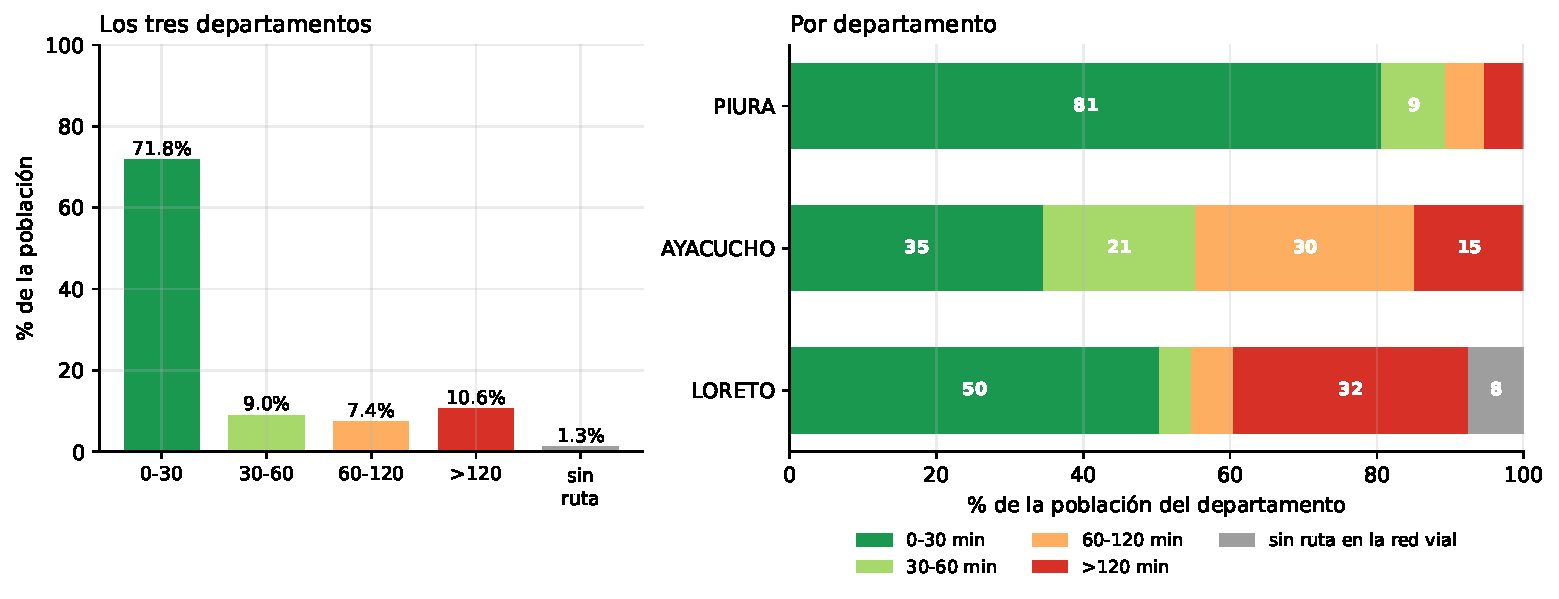
\includegraphics[width=\textwidth]{fig_cobertura_bandas.pdf}
\caption{Población por banda de tiempo de acceso. A la izquierda, el agregado
de los tres departamentos; a la derecha, la misma métrica desagregada. El
agregado está dominado por Piura, que concentra la mayor parte de la
población de la muestra.}
\label{fig:cobertura}
\end{figure}

\begin{table}[H]
\centering
\caption{Tiempo medio ponderado por población, por departamento.}
\label{tab:departamentos}
\footnotesize
\begin{tabular}{lrrrrr}
\toprule
Departamento & Tiempo medio (min) & Población con ruta & Población sin ruta & \% con ruta & Puntos \\
\midrule
LORETO & 703.1 & 608,307 & 49,811 & 92.4 & 1,024 \\
AYACUCHO & 67.2 & 328,376 & 0 & 100.0 & 2,867 \\
PIURA & 20.6 & 2,953,705 & 0 & 100.0 & 1,111 \\
\bottomrule
\end{tabular}

\end{table}

La distancia entre los tres es de otro orden de magnitud: 20.6 minutos en
Piura, 67.2 en Ayacucho y 703.1 en Loreto. Conviene además contrastar media y
mediana: la media ponderada global es de 131.2 minutos, pero la
\emph{mediana} ponderada es de \textbf{2.8 minutos}. No se contradicen: la
persona mediana de estos tres departamentos vive en una ciudad de la costa con
un hospital al lado, y la media la arrastra una cola amazónica de días de
viaje. Un titular que use solo una de las dos cifras miente por omisión.

\subsection{Distribución territorial}

\begin{figure}[H]
\centering
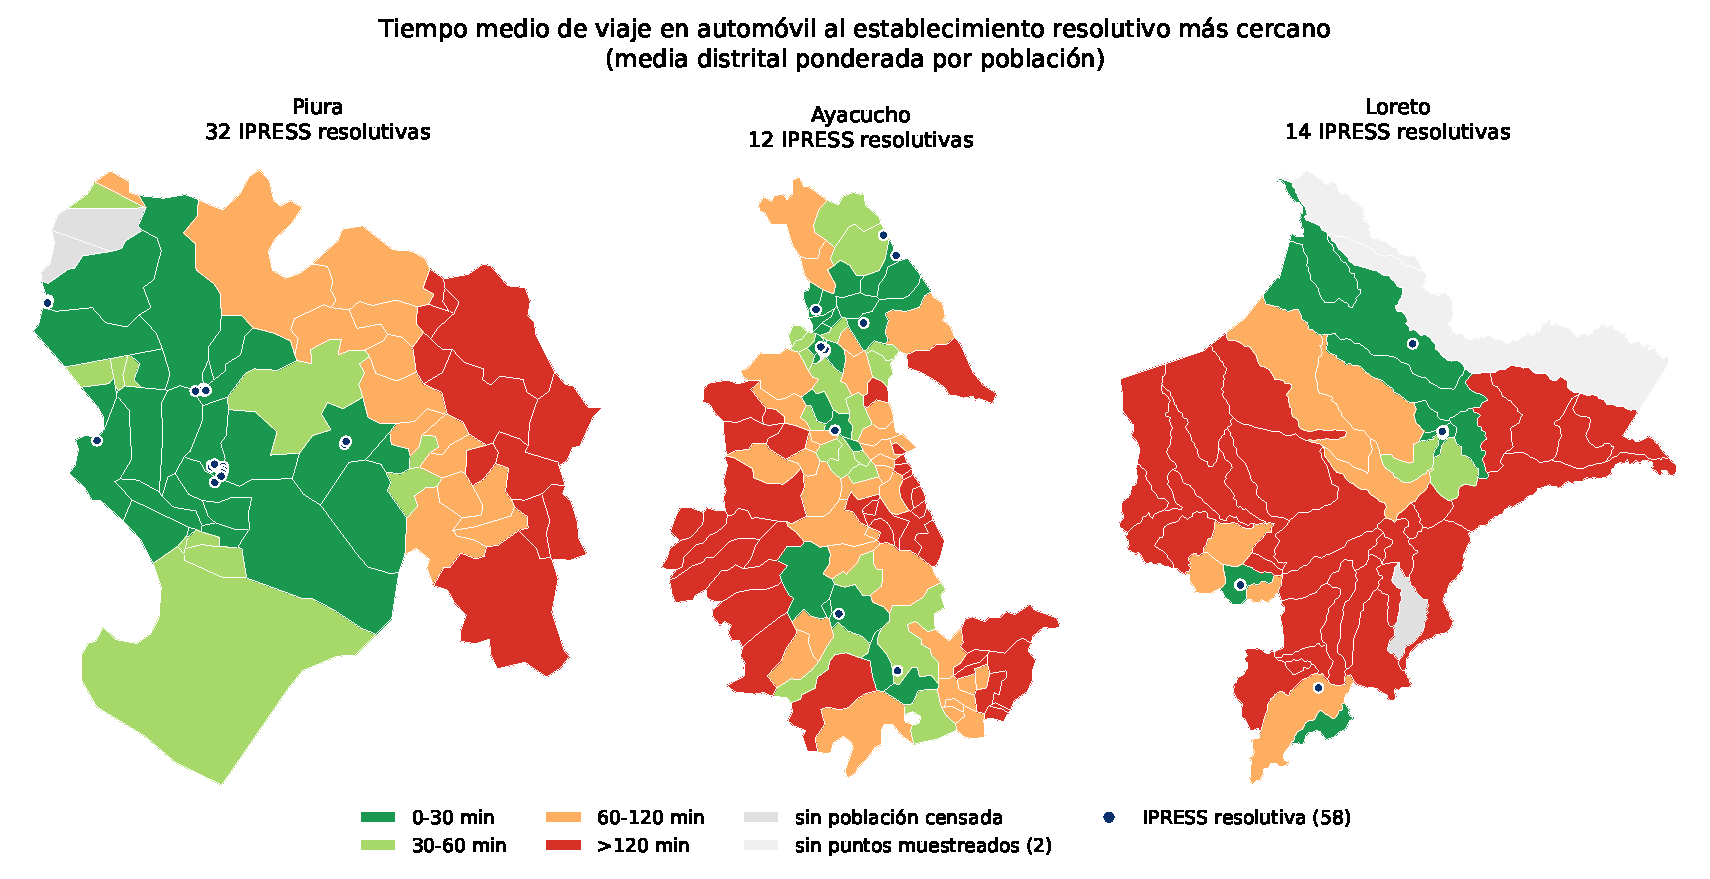
\includegraphics[width=\textwidth]{fig_mapa_acceso.pdf}
\caption{Tiempo medio distrital ponderado por población. Los distritos en gris
claro tienen ruta calculada para todos sus puntos muestreados pero ninguno de
sus centros poblados empató con el Censo 2017, de modo que no admiten media
ponderada: gris no significa mal acceso, significa ausencia de dato de
población. Los puntos azules son los 58 establecimientos resolutivos.}
\label{fig:mapa}
\end{figure}

El mapa hace visible la asimetría de la oferta: 32 de los 58 establecimientos
resolutivos están en Piura, 14 en Loreto --- un departamento casi diez veces
más extenso --- y 12 en Ayacucho. Más revelador todavía: \textbf{solo 23 de
los 237 distritos con población tienen algún establecimiento resolutivo dentro
de sus límites}. El otro 90\,\% depende enteramente de su conexión vial con el
distrito vecino.

\begin{table}[H]
\centering
\caption{Los diez distritos con peor acceso. El ranking completo de quince
está en \texttt{data/outputs/\allowbreak critical\_gap\_ranking.csv}.}
\label{tab:ranking}
\footnotesize
\begin{tabular}{rllrr}
\toprule
Puesto & Distrito & Ubigeo & Horas & Población \\
\midrule
1 & RAMON CASTILLA & 160401 & 81.8 & 40,216 \\
2 & YAVARI & 160403 & 80.5 & 5,450 \\
3 & SAN PABLO & 160404 & 64.4 & 21,618 \\
4 & YAGUAS & 160804 & 46.4 & 1,305 \\
5 & PEBAS & 160402 & 36.8 & 12,694 \\
6 & LAGUNAS & 160206 & 29.1 & 4,899 \\
7 & URARINAS & 160305 & 29.0 & 12,868 \\
8 & EMILIO SAN MARTIN & 160504 & 25.4 & 4,931 \\
9 & MAQUIA & 160505 & 22.3 & 12,036 \\
10 & LAS AMAZONAS & 160105 & 19.5 & 3,803 \\
\bottomrule
\end{tabular}

\end{table}

Los quince distritos con peor acceso están todos en Loreto, encabezados por
Ramón Castilla y Yavarí, en la frontera con Colombia y Brasil, con medias
superiores a las 80 horas. Interpretar literalmente esas 80 horas sería un
error: lo que dicen es que el trayecto por carretera es tan indirecto que deja
de describir el acceso real, que allí es fluvial. El valor del dato está en el
orden, no en la magnitud: identifica sin ambigüedad dónde la red vial no
cumple ninguna función sanitaria.

\subsection{Equidad: el acceso está concentrado}

\begin{figure}[H]
\centering
\begin{minipage}{0.52\textwidth}
\centering
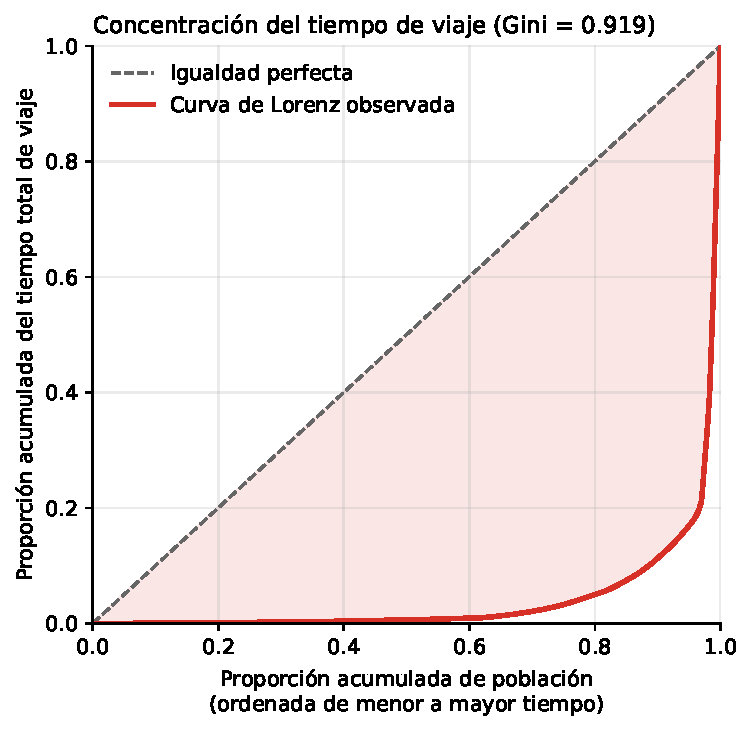
\includegraphics[width=\textwidth]{fig_lorenz.pdf}
\end{minipage}\hfill
\begin{minipage}{0.46\textwidth}
\centering
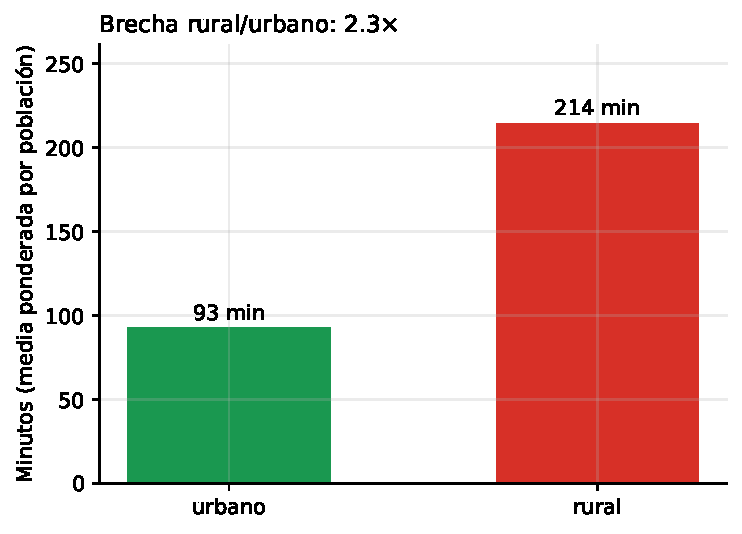
\includegraphics[width=\textwidth]{fig_urbano_rural.pdf}
\end{minipage}
\caption{Izquierda: curva de Lorenz del tiempo de viaje. Derecha: contraste
urbano/rural.}
\label{fig:equidad}
\end{figure}

El índice de Gini del tiempo de acceso es \textbf{0.919}, calculado sobre
2{,}417 puntos con tiempo y población conocidos. La interpretación correcta no
es ``el acceso es malo'' sino ``el tiempo total de viaje está extremadamente
concentrado'': la gran mayoría de la población acumula una fracción mínima del
tiempo agregado, y ese tiempo se concentra en una minoría rural y amazónica.
Dos territorios con idéntico tiempo medio pueden tener Gini muy distinto según
repartan la demora entre pocos o entre todos.

\begin{table}[H]
\centering
\caption{Contraste de acceso entre zonas urbanas y rurales.}
\label{tab:urbano-rural}
\footnotesize
\begin{tabular}{lrrrr}
\toprule
Zona & Tiempo medio (min) & Población con ruta & Población sin ruta & Puntos \\
\midrule
rural & 214.2 & 1,235,452 & 17,604 & 4,938 \\
urbano & 92.6 & 2,654,935 & 32,207 & 64 \\
\bottomrule
\end{tabular}

\end{table}

La brecha rural/urbana es de 2.3 veces (214.2 minutos frente a 92.6). Hay que
leerla con cuidado por el tamaño de los grupos: solo 64 de los 5{,}002 puntos
de la muestra son capital de algo. Que incluso el grupo ``urbano'' promedie más
de hora y media revela que la capitalidad administrativa no garantiza
proximidad a un hospital resolutivo: una capital distrital de Loreto sigue
estando a días de uno.

\subsection{El modo de viaje cambia la respuesta}

\begin{table}[H]
\centering
\caption{Tiempo al establecimiento resolutivo más cercano según modo.}
\label{tab:modos}
\footnotesize
\begin{tabular}{lrrrr}
\toprule
Modo & Puntos & Mediana (min) & P75 (min) & Veces el tiempo en automóvil \\
\midrule
Automóvil & 4,904 & 92.1 & 148.5 & -- \\
Bicicleta & 4,652 & 412.8 & 816.5 & 4.2 \\
A pie & 4,652 & 1,058.9 & 1,989.9 & 11.1 \\
\bottomrule
\end{tabular}

\end{table}

Ir a pie toma, en la mediana, 11.2 veces más que ir en automóvil; en bicicleta,
4.2 veces más. Un indicador de accesibilidad construido sobre el supuesto de
automóvil disponible describe la situación de quien tiene automóvil, no la de
la población. La comparación exigida --- a pie contra todos los
establecimientos frente a automóvil contra los resolutivos, sobre los centros
poblados urbanos --- muestra además que el establecimiento más cercano
\textbf{cambia con el modo en 84 de 234 puntos (36\,\%)}: en más de un tercio
de los casos, la política de ``derivar al establecimiento más cercano'' apunta
a un lugar distinto según cómo se viaje. Quince de esos puntos urbanos no
tienen siquiera ruta peatonal calculable.

\subsection{Altitud y acceso: una correlación que no debe leerse como causa}

\begin{figure}[H]
\centering
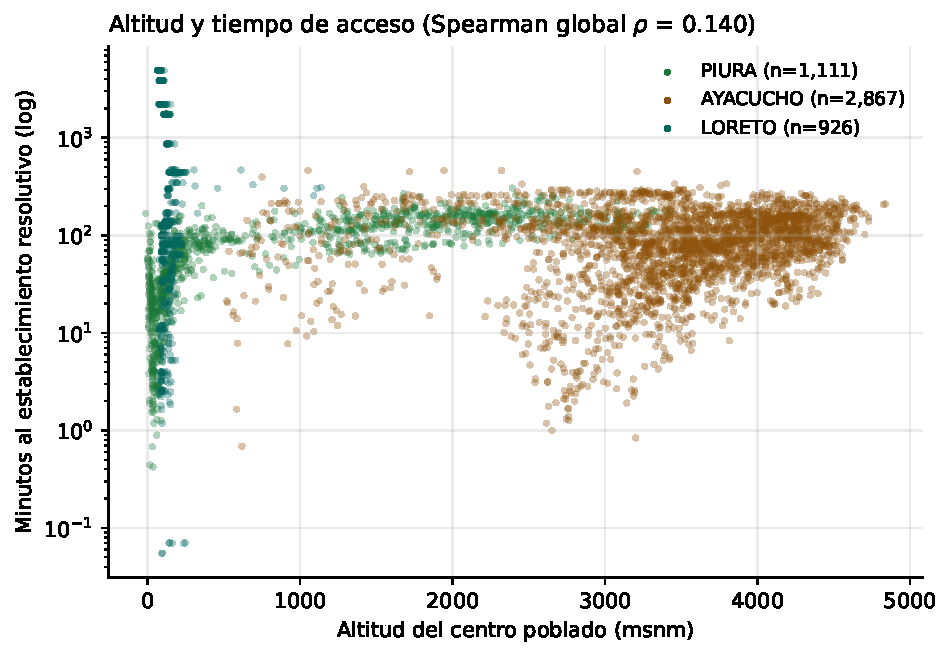
\includegraphics[width=0.82\textwidth]{fig_altitud.pdf}
\caption{Altitud del centro poblado frente a tiempo de acceso, en escala
logarítmica, por departamento.}
\label{fig:altitud}
\end{figure}

La correlación de Spearman entre altitud y tiempo de acceso es
$\rho = 0.140$ ($p < 10^{-22}$, $n = 4{,}904$): estadísticamente significativa
y sustantivamente irrelevante. La figura~\ref{fig:altitud} explica por qué.
Los peores tiempos no están en las cumbres de Ayacucho (entre 3{,}000 y
4{,}500 msnm, con tiempos concentrados alrededor de la hora y media) sino en
la Amazonía baja de Loreto (por debajo de los 200 msnm, con tiempos de miles
de minutos). De hecho, al calcular la correlación solo dentro de Loreto, el
signo se invierte ($\rho = -0.161$).

Es un caso de manual de correlación observacional entre dos efectos de una
causa común: altitud y tiempo de viaje son ambos consecuencias del relieve,
que determina la densidad de la red vial y la dispersión de la población. Con
estos datos no es posible aislar un efecto causal de la altitud, y el informe
no lo pretende. La nota correspondiente viaja dentro del propio CSV exportado,
para que no se pierda si alguien reutiliza la tabla fuera de este documento.

\subsection{Escenarios: qué compraría un ascenso de categoría}

Con el umbral de 30 minutos, el mejor candidato individual de los 607
establecimientos I-3/I-4 es el E.S. Bernal (I-4, Sechura, Piura): ascenderlo
acercaría a 141{,}446 habitantes por debajo del umbral y subiría la cobertura
del 71.8\,\% al 75.4\,\%. Pero los cinco mejores candidatos individuales están
todos en el mismo entorno de Sechura y compiten entre sí: sus ganancias
individuales suman 423{,}684 habitantes, mientras que el efecto conjunto de
los tres primeros es de 141{,}446 --- exactamente el del primero. Es la razón
por la que el panel calcula el escenario combinado en vez de sumar filas de un
ranking.

El resultado cambia por completo al filtrar. Restringido a Loreto y con umbral
de 60 minutos, el mejor candidato es el establecimiento I-4 de Caballococha,
en Ramón Castilla --- el distrito peor rankeado del estudio ---: su ascenso
movería a 34{,}988 personas por debajo de la hora y subiría la cobertura
departamental del 54.8\,\% al 60.1\,\%. Un ranking nacional ponderado por
población siempre privilegiará a la costa, donde vive la mayoría; la decisión
de a quién priorizar es política, y el panel permite hacerla explícita en vez
de esconderla en un promedio.

% ===========================================================================
\section{Discusión}
% ===========================================================================

\subsection{Línea recta contra red: por qué no basta una regla sobre el mapa}
\label{sec:recta}

Fase 2 comparó, para los 284{,}432 pares origen--destino efectivamente
enrutados, la distancia por la red contra la distancia en línea recta
(figura~\ref{fig:recta}, tabla~\ref{tab:calibracion}).

\begin{figure}[H]
\centering
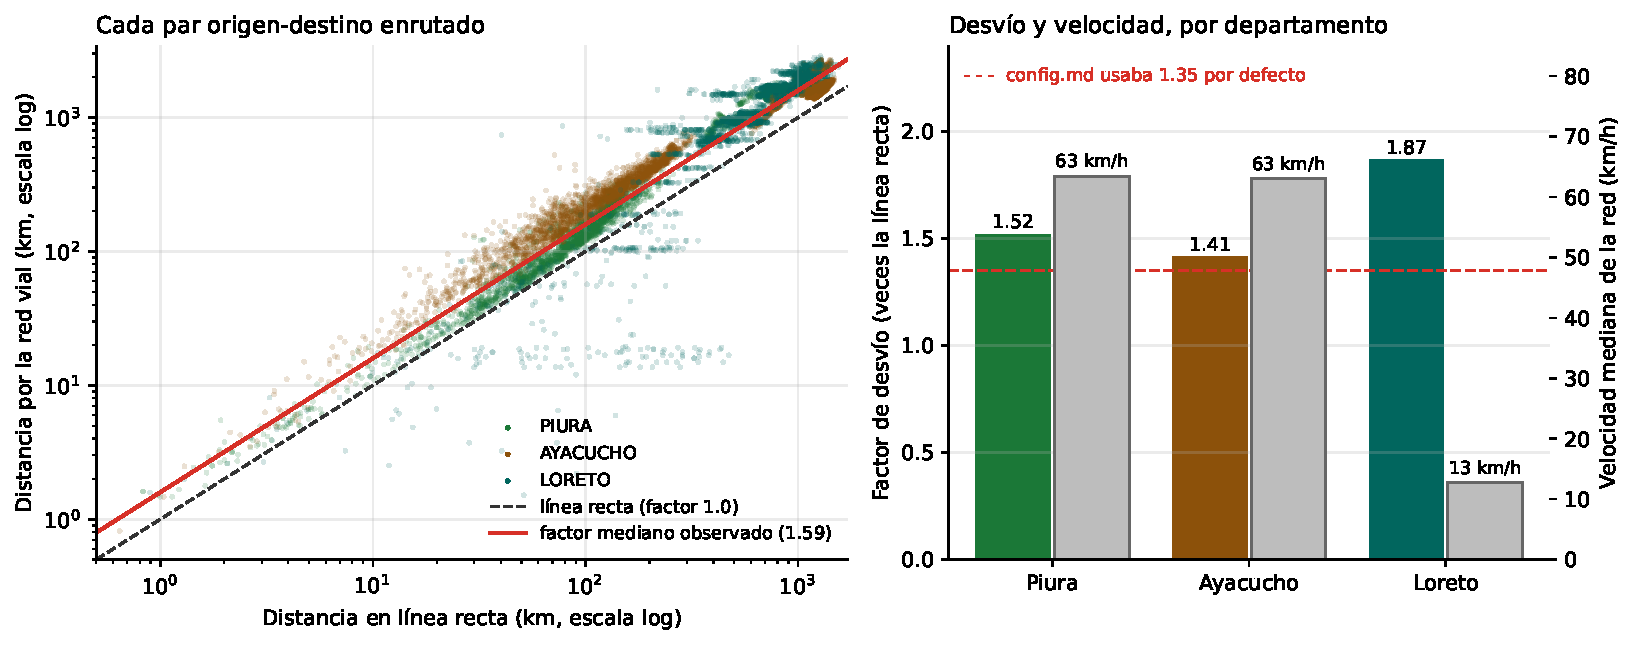
\includegraphics[width=\textwidth]{fig_recta_vs_red.pdf}
\caption{Izquierda: distancia por la red frente a distancia en línea recta,
para una muestra de 20{,}000 pares enrutados. Derecha: factor de desvío
mediano y velocidad mediana de la red, por departamento.}
\label{fig:recta}
\end{figure}

\begin{table}[H]
\centering
\caption{Calibración empírica de la relación entre distancia de red y
distancia en línea recta.}
\label{tab:calibracion}
\footnotesize
\begin{tabular}{lrrrrr}
\toprule
Departamento & Pares enrutados & Desvío P25 & Desvío mediano & Desvío P75 & Velocidad mediana (km/h) \\
\midrule
AYACUCHO & 166,280 & 1.30 & 1.41 & 1.92 & 63.0 \\
LORETO & 53,567 & 1.67 & 1.87 & 2.07 & 12.7 \\
PIURA & 64,428 & 1.34 & 1.52 & 1.89 & 63.4 \\
TODOS & 284,432 & 1.32 & 1.59 & 1.93 & 62.0 \\
\bottomrule
\end{tabular}

\end{table}

Tres conclusiones se desprenden de ahí. Primera: el factor de desvío mediano
es \textbf{1.59}, muy por encima del 1.35 que \texttt{config.md} traía como
valor por defecto; usar el valor supuesto habría subestimado
sistemáticamente las distancias del respaldo. Segunda: el factor no es
constante entre territorios --- 1.41 en Ayacucho, 1.52 en Piura, 1.87 en
Loreto ---, de modo que un único factor nacional mezcla realidades distintas.
Tercera, y la más importante: \textbf{el problema amazónico no es
principalmente la forma de la red, sino su velocidad}. Loreto desvía un
32\,\% más que Ayacucho, pero se recorre a 12.7 km/h medianos frente a los
63 km/h de la sierra y la costa. Combinando ambos efectos, un kilómetro en
línea recta cuesta 1.3 minutos en Ayacucho y 9.8 minutos en Loreto: siete
veces más. Cualquier estimación de accesibilidad basada en distancia
euclidiana, con o sin factor de corrección, es inservible en la Amazonía.

\subsection{Tres conclusiones sustantivas}

\textbf{El problema no es la cantidad de establecimientos, es su categoría y
su distribución.} Los tres departamentos tienen 2{,}844 establecimientos
georreferenciados, pero solo 58 son resolutivos. El primer nivel existe y está
razonablemente distribuido; lo que falta es capacidad resolutiva a distancia
razonable. Una política que mida ``acceso a un establecimiento de salud'' sin
distinguir categoría reportará una cobertura excelente sobre un problema
intacto.

\textbf{En Loreto, medir el acceso por carretera es medir la cosa
equivocada.} El 38\,\% de centros poblados sin vía a menos de un kilómetro, el
8\,\% de población sin ninguna ruta y las medias de más de 80 horas son la
constatación cuantitativa de que el transporte relevante allí es fluvial. Este
trabajo no puede medir el acceso real amazónico, y decirlo con claridad es más
útil que producir un número verosímil pero falso.

\textbf{La desigualdad es más informativa que el promedio.} Un Gini de 0.919
indica que el sistema funciona bien para la mayoría y muy mal para una minoría
identificable geográficamente. Esa minoría no aparece en ningún promedio
departamental, pero salta de inmediato en el ranking distrital, que es la
unidad sobre la que efectivamente se asignan presupuestos.

% ===========================================================================
\section{Limitaciones}
% ===========================================================================

Ordenadas por su capacidad de alterar las conclusiones.

\begin{enumerate}[leftmargin=1.4em]

\item \textbf{El modelo no representa el transporte fluvial.} Es la limitación
dominante. OSRM enruta sobre la red vial de OpenStreetMap; los ríos
amazónicos, que son las vías reales de Loreto, no están en esa red. Todos los
tiempos de Loreto deben leerse como ``tiempo por carretera si existiera''.
Corregirlo exigiría una red fluvial navegable con velocidades por tipo de
embarcación, que no existe como dato abierto para el Perú.

\item \textbf{La cobertura de OpenStreetMap está sesgada contra lo rural.} OSM
es cartografía voluntaria: las ciudades están mapeadas con detalle y las
trochas rurales, de forma irregular. El 38\,\% de puntos sin vía a menos de un
kilómetro mezcla dos fenómenos que estos datos no permiten separar: caminos
que no existen y caminos que existen pero nadie ha mapeado. En el primer caso
el tiempo reportado es correcto; en el segundo es pesimista. El sesgo empuja
en la dirección de exagerar la brecha rural, y no se puede acotar sin
verificación de campo.

\item \textbf{El 23.45\,\% de los establecimientos no tiene coordenadas.} Se
excluyeron del enrutamiento 872 de 3{,}718 registros. Si estuvieran
distribuidos como los demás, el sesgo sería pequeño; si se concentraran en
zonas periféricas --- lo más probable, porque el registro se completa mejor en
establecimientos grandes y urbanos ---, los tiempos aquí reportados serían
\emph{pesimistas} en esas zonas. No es posible determinar la dirección del
sesgo con la información disponible.

\item \textbf{El modelo mide distancia-tiempo, no atención.} Un establecimiento
resolutivo abierto en el registro puede no tener especialista, insumos, banco
de sangre o cama disponible en el momento de la emergencia. RENIPRESS es un
registro administrativo autodeclarado y no un censo de capacidad instalada
verificada. El acceso geográfico es condición necesaria, no suficiente.

\item \textbf{No se modela la disponibilidad de ambulancias ni de transporte
de emergencia.} Todos los tiempos suponen que existe un vehículo listo en el
centro poblado en el momento del evento. En la práctica, buena parte de la
población rural no dispone de vehículo propio y depende de una ambulancia que
debe primero \emph{ir} desde el establecimiento --- lo que en la práctica
duplica el tiempo --- o de transporte informal con disponibilidad incierta. Los
tiempos de este informe son, en ese sentido, un límite inferior optimista.

\item \textbf{390 establecimientos no tienen categoría legible} y quedaron
clasificados como \texttt{SIN\_\allowbreak CATEGORIA}, o sea, no resolutivos. Si alguno
fuera en realidad de categoría II o III, el tiempo de acceso de su entorno
estaría sobreestimado. Es un sesgo en una sola dirección: por esta causa los
tiempos reportados nunca son mejores de lo real, solo peores.

\item \textbf{La población está incompleta en el 35.6\,\% de los centros
poblados.} Las métricas ponderadas describen a la población \emph{con
población conocida}, no al total. Seis distritos --- entre ellos Veintiséis de
Octubre (Piura) y San Juan Bautista (Ayacucho), ambos urbanos y densamente
poblados --- quedan sin media ponderable por esta causa.

\item \textbf{La expansión por pesos de muestreo sobreestima la población
total en un 17\,\%}: 3{,}940{,}199 habitantes frente a los 3{,}356{,}495 del
directorio del INEI. La causa es que dentro de cada distrito el muestreo fue
uniforme, no proporcional a la población, y los centros poblados que sí
empataron con el Censo tienden a ser más grandes que el promedio de su
distrito. Los \emph{porcentajes} por banda son robustos a este sesgo, porque
afecta a numerador y denominador; los \emph{niveles absolutos} de población
deben leerse como órdenes de magnitud.

\item \textbf{La muestra cubre el 25.7\,\% de los centros poblados.} La
estratificación garantiza que ningún distrito quede fuera, pero dentro de cada
distrito la selección fue aleatoria uniforme. Los intervalos de confianza de
las medias distritales con pocos puntos muestreados son amplios; el informe no
los reporta y esa es una deuda metodológica declarada.

\item \textbf{Los tiempos del simulador de escenarios son estimados, no
enrutados.} La matriz OD se calculó contra los 58 establecimientos
resolutivos, no contra los 607 candidatos a ascenso; mientras no se recalcule
con OSRM, el simulador estima esos tiempos con la calibración de la
sección~\ref{sec:recta}. Sirve para comparar y priorizar candidatos, no para
prometer un tiempo concreto a un centro poblado concreto.

\item \textbf{El proxy urbano/rural es administrativo.} No es la definición del
INEI. Una capital distrital amazónica de doscientos habitantes queda
clasificada como urbana, y un centro poblado grande conurbado con una capital
queda como rural. La brecha de 2.3 veces es, estrictamente, una comparación
entre capitales y no capitales.

\item \textbf{Los tiempos de OSRM son de flujo libre.} No modelan congestión,
estado de la vía ni época de lluvias. En sierra y selva, una vía afirmada en
temporada de lluvias puede ser intransitable durante semanas.

\end{enumerate}

% ===========================================================================
\section{Conclusiones y recomendaciones}
% ===========================================================================

\begin{enumerate}[leftmargin=1.4em]
\item El 71.8\,\% de la población estimada alcanza un establecimiento
resolutivo en menos de 30 minutos por carretera, pero ese promedio agrega
realidades incomparables: 81\,\% en Piura, 35\,\% en Ayacucho y 50\,\% en
Loreto, con un 32\,\% adicional a más de dos horas. 708{,}676 personas están a
más de una hora.

\item La desigualdad del acceso (Gini 0.919) es tan informativa como el nivel
promedio y ubica el problema en una minoría geográficamente identificable: los
distritos fronterizos y ribereños de Loreto.

\item Solo 23 de 237 distritos cuentan con un establecimiento resolutivo
propio. La política relevante no es construir más postas, sino elevar la
capacidad resolutiva de establecimientos existentes en nodos bien conectados.
El simulador cuantifica esa decisión: un solo ascenso en Caballococha subiría
la cobertura a una hora de Loreto en 5.3 puntos porcentuales.

\item Para Loreto, cualquier indicador de accesibilidad basado en red vial es
inadecuado por construcción. La recomendación metodológica es explícita: antes
de invertir en más modelamiento vial de la Amazonía, hay que producir el dato
que falta, una red fluvial navegable con velocidades por tipo de embarcación.

\item El modo de viaje importa: a pie los tiempos se multiplican por 11 y en un
tercio de los casos cambia cuál es el establecimiento más cercano. Los
indicadores oficiales de accesibilidad deberían declarar el modo que suponen.

\item Recomendación operativa sobre los datos: publicar RENIPRESS con
coordenadas completas y categoría normalizada, y exponer la capa de centros
poblados de SIGMED con una API y una licencia declarada. Un cuarto de la
oferta hoy es invisible para cualquier análisis geográfico.
\end{enumerate}

\textbf{Reproducibilidad.} El repositorio se reproduce ejecutando en orden
\texttt{src.acquisition} y los cinco guiones \texttt{run\_\allowbreak
fase1} a \texttt{run\_\allowbreak fase5}; solo la Fase 2 necesita OSRM en
Docker, porque las Fases 4 y 5 consumen las matrices ya versionadas. El panel
se levanta con \texttt{streamlit run app.py} y la suite de pruebas
(\texttt{pytest -m 'not osrm'}) cubre las reglas de validación, las métricas,
el simulador y el contrato entre el panel y \texttt{src/metrics.py}. Ningún
parámetro está escrito dentro del código: todos viven en \texttt{config.md}.

% ===========================================================================
\begin{thebibliography}{9}
\footnotesize

\bibitem{osrm}
Luxen, D. y Vetter, C. (2011).
\emph{Real-time routing with OpenStreetMap data}.
Proceedings of the 19th ACM SIGSPATIAL International Conference on Advances in
Geographic Information Systems, pp. 513--516.

\bibitem{lorenz}
Lorenz, M. O. (1905).
\emph{Methods of measuring the concentration of wealth}.
Publications of the American Statistical Association, 9(70), pp. 209--219.

\bibitem{gini}
Gini, C. (1912). \emph{Variabilità e mutabilità}. Bologna: Tipografia di Paolo
Cuppini.

\bibitem{renipress}
SUSALUD. \emph{Registro Nacional de Instituciones Prestadoras de Servicios de
Salud (RENIPRESS)}. Portal Nacional de Datos Abiertos del Perú. Licencia
ODC-By. \url{https://www.datosabiertos.gob.pe}

\bibitem{sigmed}
MINEDU. \emph{Sistema de Información Geográfica de la Educación (SIGMED), capa
de centros poblados}. \url{https://sigmed.minedu.gob.pe/descargas/}

\bibitem{inei}
INEI (2018). \emph{Directorio Nacional de Centros Poblados. Censos Nacionales
2017: XII de Población, VII de Vivienda y III de Comunidades Indígenas}.
Publicación Lib1541.

\bibitem{osm}
OpenStreetMap contributors (2026). \emph{Extracto de Perú}. Geofabrik.
Licencia ODbL 1.0.
\url{https://download.geofabrik.de/south-america/peru-latest.osm.pbf}

\bibitem{geojson}
Repositorio \texttt{juaneladio/\allowbreak peru-geojson}: límites
departamentales, provinciales y distritales del Perú derivados de la
cartografía censal del INEI (2007). Licencia MPL-2.0.
\url{https://github.com/juaneladio/peru-geojson}

\end{thebibliography}

\end{document}
